\documentclass[5p]{elsarticle} % seleccionar: preprint, review, 1p, 3p, 5p



\usepackage{mathtools}
\journal{ }


%to force all images and table in one single section
\usepackage{placeins}
% It is necesary to add \FloatBarrier in the text. 
% After that order, all the floating are shown.

%%%%%%%%%%%%%%%%%%%%%%%
%% Elsevier bibliography styles
%%%%%%%%%%%%%%%%%%%%%%%
%% To change the style, put a % in front of the second line of the current style and
%% remove the % from the second line of the style you would like to use.
%%%%%%%%%%%%%%%%%%%%%%%

%% Numbered
%\bibliographystyle{model1-num-names}

%% Numbered without titles
%\bibliographystyle{model1a-num-names}

%% Harvard
%\bibliographystyle{model2-names.bst}\biboptions{authoryear}

%% Vancouver numbered
%\usepackage{numcompress}\bibliographystyle{model3-num-names}

%% Vancouver name/year
%\usepackage{numcompress}\bibliographystyle{model4-names}\biboptions{authoryear}

%% APA style
%\bibliographystyle{model5-names}\biboptions{authoryear}

%% AMA style
%\usepackage{numcompress}\bibliographystyle{model6-num-names}

%% `Elsevier LaTeX' style
\bibliographystyle{elsarticle-num}

%%%%%%%%%%%%%%%%%%%%%%%
\hyphenation{}
\usepackage{eurosym}
\usepackage{threeparttable} % allow the use of footnote within tables

\usepackage{url}
\usepackage[colorlinks=true, citecolor=blue, linkcolor=blue, filecolor=blue,urlcolor=blue]{hyperref}

%to add the number to the lines
\usepackage{lineno}
\modulolinenumbers[5]

\usepackage{lineno,hyperref}
\modulolinenumbers[1]
\usepackage{amsmath}
\usepackage{siunitx}
\usepackage{eurosym}
\biboptions{numbers,sort&compress}
\usepackage[europeanresistors,americaninductors]{circuitikz}
\usepackage{adjustbox}
\usepackage{xspace}
\usepackage{caption}
\usepackage{booktabs}
\usepackage{tabularx}
\usepackage{threeparttable}
\usepackage{multicol}
\usepackage{float}
\usepackage{graphicx,dblfloatfix}
\usepackage{csvsimple}
%% new commands
\newcommand{\ubar}[1]{\text{\b{$#1$}}}
\newcommand*\OK{\ding{51}}
%\renewcommand*\nompostamble{\end{multicols}}
\newcommand{\specialcell}[2][c]{%
	\begin{tabular}[#1]{@{}l@{}}#2\end{tabular}}
\def\co{CO${}_2$}
\def\el{${}_{\textrm{el}}$}
\def\th{${}_{\textrm{th}}$}


%\renewcommand*{\today}{July, 10 2018}
%\hypersetup{draft} %to avoid problems with hyperref while drafting

\begin{document}

\begin{frontmatter}

\title{The benefits of ambitious short-term targets when decarbonising the coupled electricity and heating energy system in Europe}

%\author[mymainaddress,iClimate]{Marta Victoria\corref{mycorrespondingauthor}}
%\ead{mvp@eng.au.dk}
%\author[mymainaddress]{Kun Zhu}
%\author[kitaddress]{Tom Brown}
%\author[mymainaddress,iClimate]{Gorm B. Andresen}
%\author[mymainaddress,iClimate]{Martin Greiner}
%\cortext[mycorrespondingauthor]{Corresponding author}
%\address[mymainaddress]{Department of Engineering, Aarhus University, Inge Lehmanns Gade 10, 8000 Aarhus, Denmark}
%\address[iClimate]{iCLIMATE Interdisciplinary Centre for Climate Change, Aarhus University}
%\address[kitaddress]{Institute for Automation and Applied Informatics (IAI), Karlsruhe Institute of Technology (KIT), Forschungszentrum 449, 76344, Eggenstein-Leopoldshafen, Germany}



\begin{abstract}

It is now clear that urgent actions are needed to mitigate climate change and a CO$_2$-neutral society must be attained by 2050. The open question is how to transition towards that society in a way that is effective, fast, and fair. In a context of increasing public awareness, discussions on the possibility of increasing CO$_2$ reduction targets for Europe have started. Here, we model alternative transition paths with equivalent emissions budget for the sector-coupled networked European energy system. We show that ambitious CO$_2$ reductions in the short term not only trigger a cheaper transition but also incentivise smoother built rates for the required new capacities which could be beneficial for local economies and jobs creation.

\end{abstract}

\begin{keyword}

%storage, energy system modelling, sector coupling, grid integration of renewables, transmission grid, CO2 emission targets

%\texttt{elsarticle.cls}\sep \LaTeX\sep Elsevier \sep template
%\MSC[2010] 00-01\sep  99-00
\end{keyword}

\end{frontmatter}

\linenumbers

Achieving a climate-neutral European Union in 2050 \cite{in-depth_2018} requires meeting the in-between milestones. Although carbon emissions will most probably curb by 20\% in 2020, relative to 1990 \cite{EEA_totalGHG}, it is unclear whether this will be the case for the -40\% objective settled for 2030. The national energy plans for the coming decade submitted by member states do not add up the necessary reduction to meet the target \cite{EU-appraisal_2019}, while in the context of a \textit{European Green Deal} a more ambitious reduction of -55\% is currently under discussion \cite{GreenDeal}. At the same time and led by young people \cite{Warren_2019}, society is claiming for more ambitious climate actions \cite{Rinscheid_2019}. Electricity generation is expected to spearhead the transition spurred by the dramatic cost reduction of wind \cite{Lantz_2012} and solar photovoltaics (PV) \cite{Creutzig_2017, Haegel_2019}. A vast body of literature shows that a power system based on wind, solar, and hydro generation can supply hourly electricity demand in Europe as long as proper balancing is provided 
\cite{Eriksen_2017, Schlachtberger_2017, Gils_2017a, Brown_response}. This can be done reinforcing interconnections among neighbouring countries \cite{Rodriguez_2014} to smooth renewable fluctuations by regional aggregation or through temporal balancing using local storage \cite{Rasmussen_2012, Cebulla_2017}. Moreover, coupling the power system with other sectors such as heating or transport could provide additional flexibilities facilitating the system operation and simultaneously helping to abate emissions in those sectors \cite{Connolly_2016, Brown_2018, Child_2019}. 

CO$_2$ emissions from heating in residential and services sector show a more modest historical reduction trend than electricity generation (Fig. \ref{fig_carbon_budget}). Nordic countries have been particularly successful in reducing carbon emissions from the heating sector by using sector-coupling strategies (Supplementary Note 3). Denmark, where more than half of the households are connected to district heating systems \cite{Gross_2019}, has shifted the fuel used in Central Heat and Power (CHP) units from coal to biomass and urban waste incineration \cite{DEA_2015}. The high penetration of heat pumps in Sweden can be explained by a path-dependence process \cite{Gross_2019} and it is now supported by high CO$_2$ prices \cite{Carbon_pricing_2019} and low electricity taxes. 

Greenfield optimisation of the future European energy system, that is, building the system from scratch, shows that sector-coupling decreases the system cost and reduces the need for extending transmission lines due to the additional local flexibility brought by heating and transport sectors \cite{Brown_2018}. Sector-coupling allows further CO$_2$ reductions before large capacities of storage become necessary, providing more time to develop further storage technologies \cite{Victoria_2019_storage}. Greenfield optimisation is useful to investigate the optimal configuration of the fully-decarbonised system, but it does not provide insights on how to transition towards it. Today's generation fleet and decisions taken in intermediate steps will shape the final configuration. 
Alternative transition paths for the European power system have been analysed using myopic optimisation, without full foresight over the investment horizon \cite{Bogdanov_2019, Plesmann_2017, Gerbaulet_2019, Poncelet_2016}. Myopic optimisation results in higher cumulative system cost than optimising the entire transition period with perfect foresight because the former leads to stranded investments \cite{Gerbaulet_2019, Heuberger_2018}. However, the myopic approach is less sensitive to the assumed discount rate and can capture better short-sighted behaviour of political actors and investors. 

Here, we use a sector-coupled networked model of the European energy system and myopic optimisation in 5-years steps from now to 2050 to investigate the impact of different CO$_2$ restriction paths with the same carbon budget. In every time step, the expansion of generation, storage, and interconnection capacities in every country is allowed  if it results cost effective under the corresponding global emissions constraint. We show that a transition path with more ambitious short-term CO$_2$ targets reduces the cumulative system cost and requires more stable build rates, which are beneficial from the point of view of social acceptance, local industry, and jobs creation. Compared to existing transition paths analyses for the European power system \cite{Plesmann_2017, Gerbaulet_2019, Poncelet_2016}, our research includes the coupling with the heating \textcolor[rgb]{1,0,0}{(and transport)} sector. The use of alternative CO$_2$ reduction paths with constant cumulative emissions is also a novelty of this work. 

Integrated Assessment Models (IAMs) with similar spatial resolution than our model, i.e., one node per country, have also been used to model the sector-coupled decarbonization of Europe \cite{in-depth_2018, JRC-EU-TIMES, Creutzig_2017}. However, IAMs typically use a much lower time resolution, \textit{e.g.} using a few time slices to represent a full year \cite{JRC-EU-TIMES, Loffler_2019, Poncelet_2016, McGlade_2015, Babrowski_2014} or considering the residual load duration curve \cite{Creutzig_2017, Ueckerdt_2017}. The hourly resolution in our model unveils several effects that are critical to the operation of highly renewable systems, such as the solar and wind non-correlations smoothed by the grid, the role of long-term storage, and the system operation during cold spells, \textsl{i.e.} a cold week with low wind and solar generation. By using an open model, we ensure transparency and reproducibility of the results in a  discipline with high policy relevance such as it is energy modelling \cite{Pfenninger_2017, Pfenninger_2018}. 

\paragraph{\textbf{Carbon budget for electricity and heating in Europe}} \

A remaining global carbon budget of 800 Gigatons (Gt) of CO$_2$ can be emitted from 2018 onwards to limit the anthropogenic warming to 1.75$^{\circ}$C relative to preindustrial period with a probability of greater than 66\% \cite{IPCC_1.5}. Different sharing principles can be used to split the global carbon budget into regions and countries \cite{Raupach_2014}. We consider an equal per-capita distribution that translates into a quota of 48 GtCO$_2$ for Europe. Since the historical quota has been much higher this implies that Europe must be more ambitious than other regions. Assuming that sectoral distribution of emissions within Europe remains at present values, the carbon budget for the generation of electricity and provision of heating in the residential and services sector accounts for approximately 21 GtCO$_2$, \cite{UNFCCC_inventory} and Supplementary Note 2. %Figueres_2017, blog_budget

\begin{figure}[!h]
\centering
	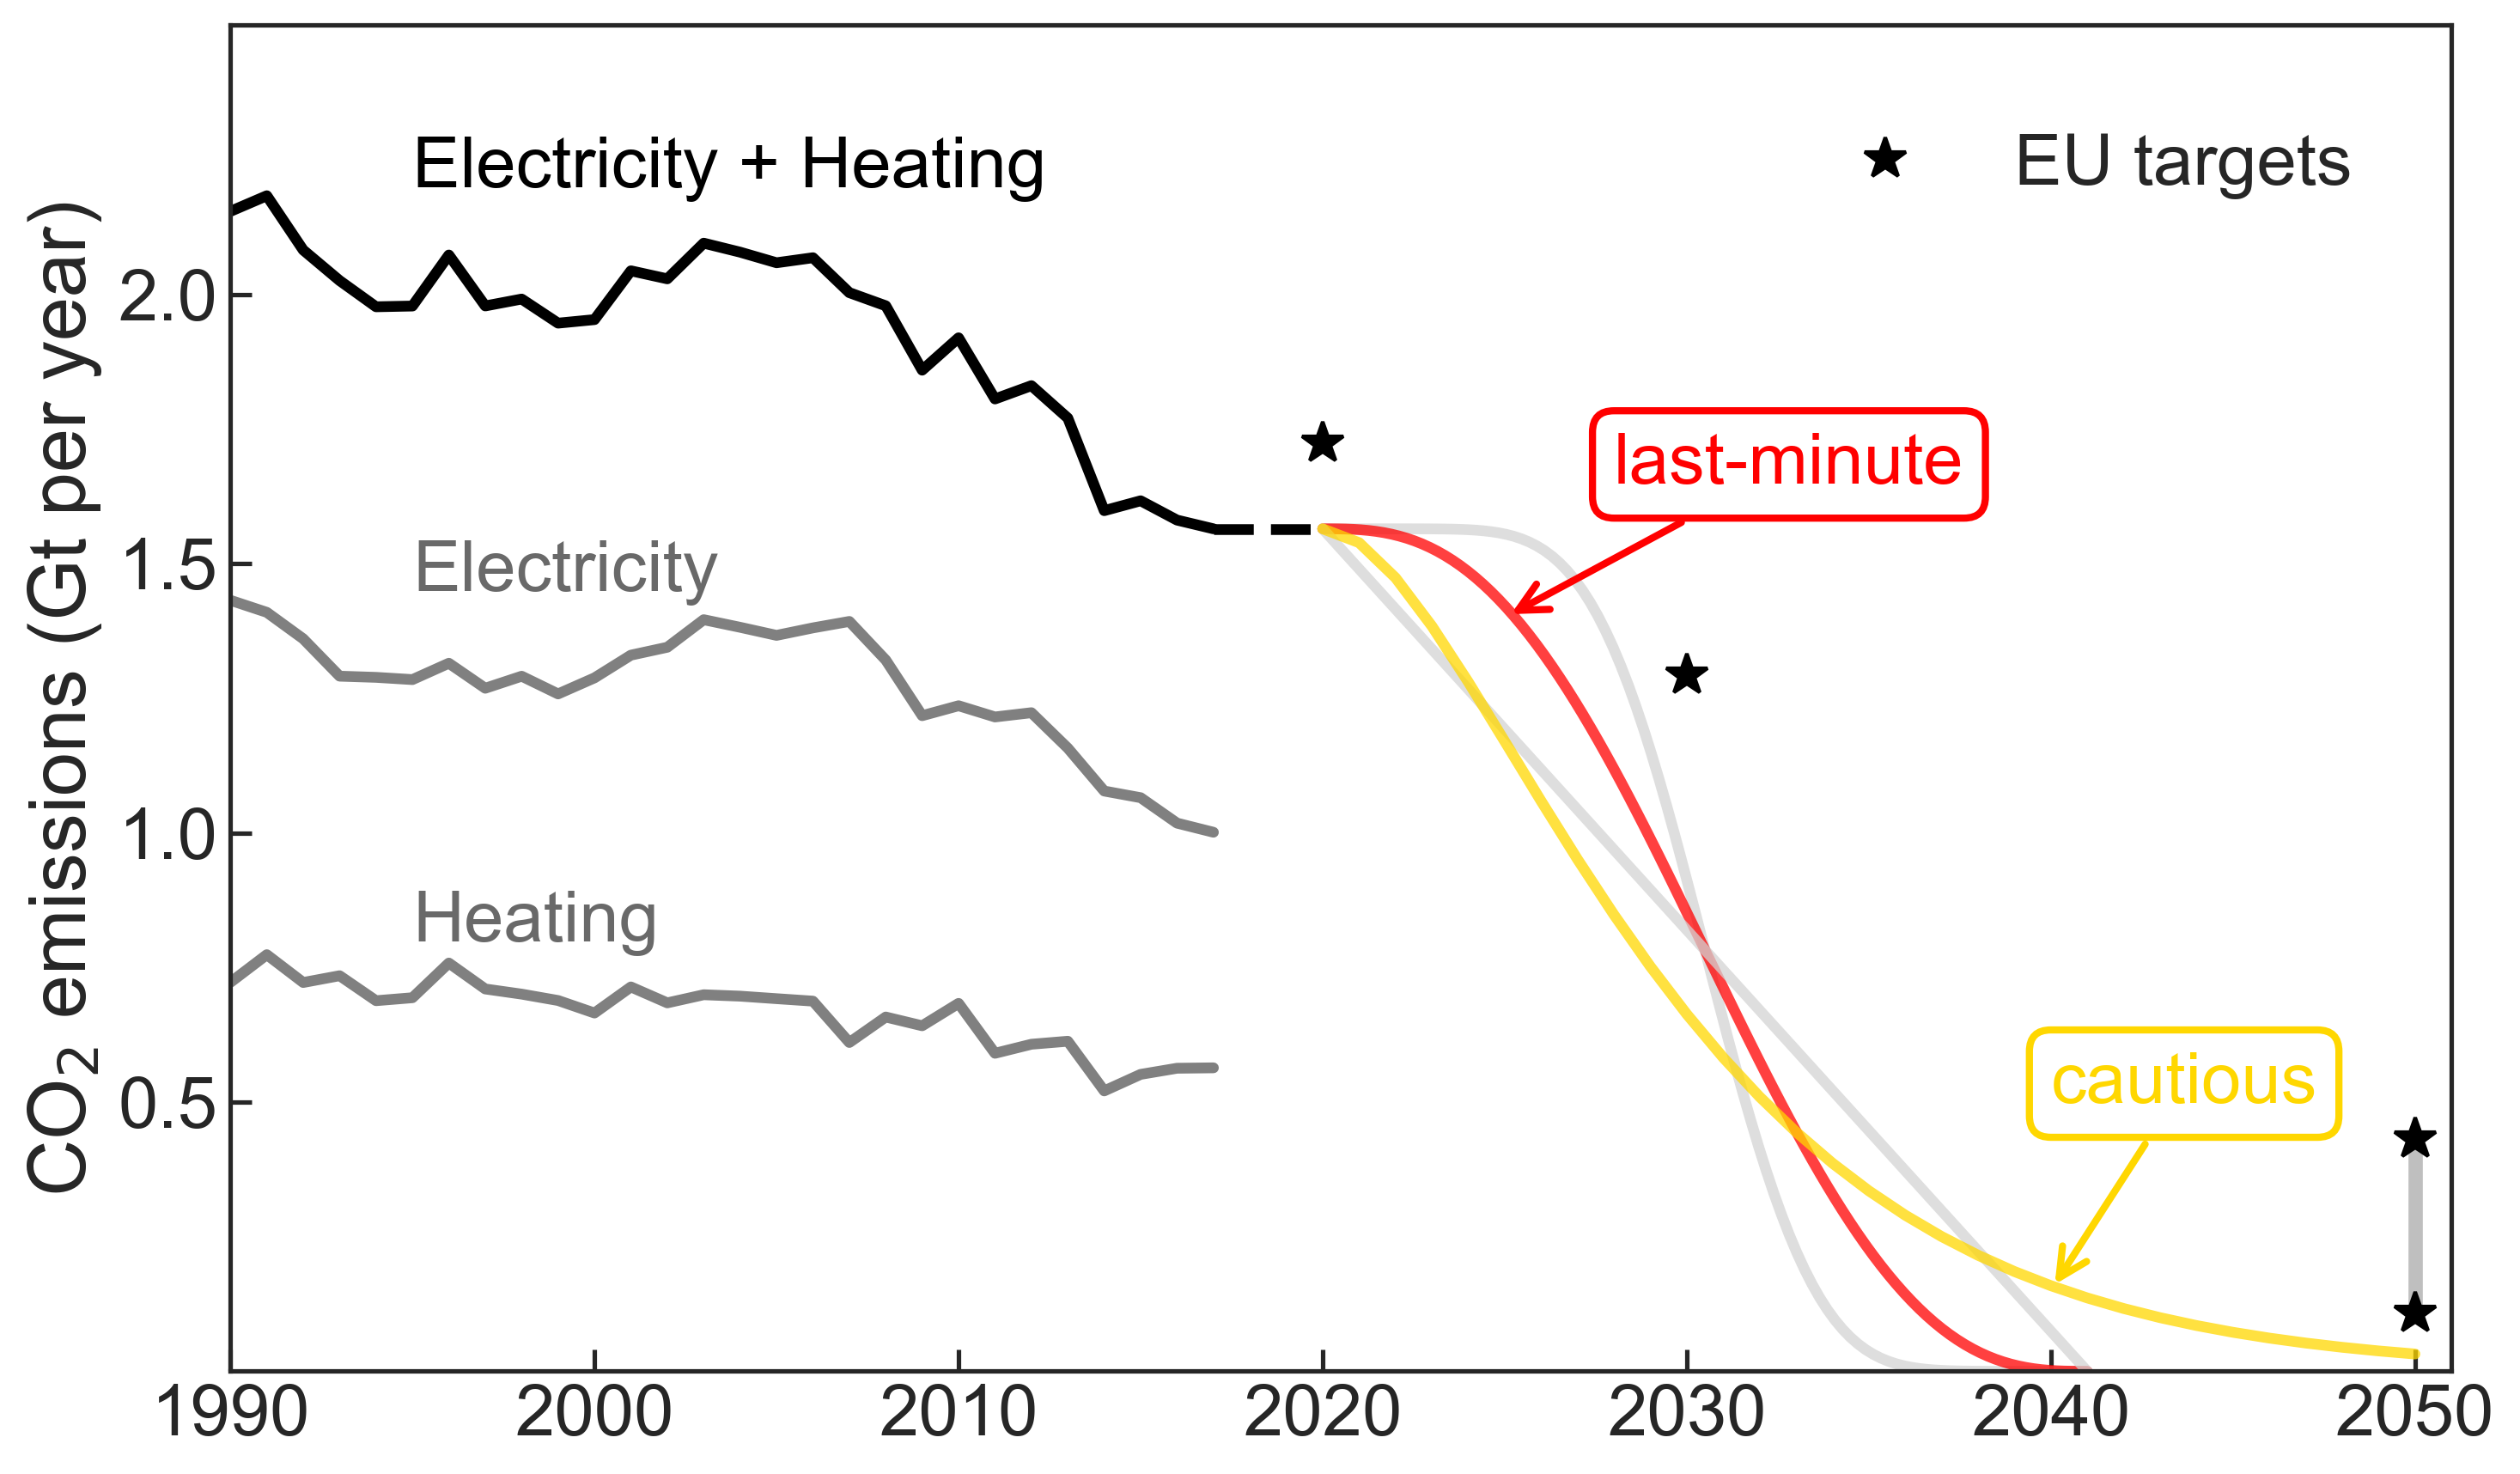
\includegraphics[width=\columnwidth]{figures/carbon_budget.png}
\caption{Historical CO$_2$ emissions from the European power system and heating supply in the residential and services sectors \cite{UNFCCC_inventory}. The various future transition paths shown in the figure have the same cumulative CO$_2$ emissions, which correspond to the remaining 21 Gt CO$_2$ budget to avoid human-induced warming above 1.75$^{\circ}$C with a probability of greater than 66\%, assuming current sectoral distribution for Europe, and equity sharing principle among regions. Black stars indicate committed EU reduction targets, while white stars mark under-discussion target.} \label{fig_carbon_budget} 
\end{figure}

\paragraph{\textbf{Stranded assets}} \

Here we investigate the consequences of following two alternative transition paths. As in Aesop's fable, the Tortoise pathway represents a cautious approach in which significant emissions reduction are attained in early years. In the Hare pathway, the low initial reduction targets quickly deplete the carbon budget requiring a sharp reduction later. The two alternative paths arrive at a similar system configuration in 2050. Only in the later years, under heavy CO$_2$ restriction, balancing technologies appear in the system. They include large storage capacities comprising electric batteries and H$_2$ storage, methanation, and reinforced interconnections.  Cumulative cost for the Tortoise path represents 7,800 billion euros (B\EUR), while the Hare path accounts for 8,100 B\EUR. OCGT and CCGT gas power plants represent the main stranded assets causing the higher cost in the later. The higher CO$_2$ emissions allowance in 2030 and earlier allow the installation of such plants. However, the drastic change in emissions restriction in subsequent years, avoids the operation of gas power plants. The Europe-averaged utilisation factors shown in Fig. \ref{fig_utilisation_factors} are close to zero from 2040 onwards for the gas units in the Hare path, and they recover less than \textcolor[rgb]{1,0,0}{X\%} of their cost via market revenues. For both transition paths, even in the initial years the utilisation factor of gas is below 50\%. This is a consequence of the role that gas units play as backup technology securing electricity and heat supply when there is a significant deficit of renewable generation, but it is also a consequence of the large capacity of gas recently installed in Europe. The pyramid age of existing electricity generation technologies in Europe, Fig. \ref{fig_age_distribution}, unveils that most of the `younger' power plants use gas. Since most of the gas capacity in Europe was installed less than 25 years ago, part of this capacity represent a stranded asset during the initial years for both transition paths. Although, infrautilisation of existing generation capacity might be seen as an unnecessary contribution to higher cost of energy it must be remarked that the early retirement of electricity infrastructure has been identified as one of the most cost-effective actions to reduce committed emissions and enable a 2$^{\circ}$C-compatible future evolution of global emissions \cite{Tong_2019}.

\begin{figure*}[!h]
\centering
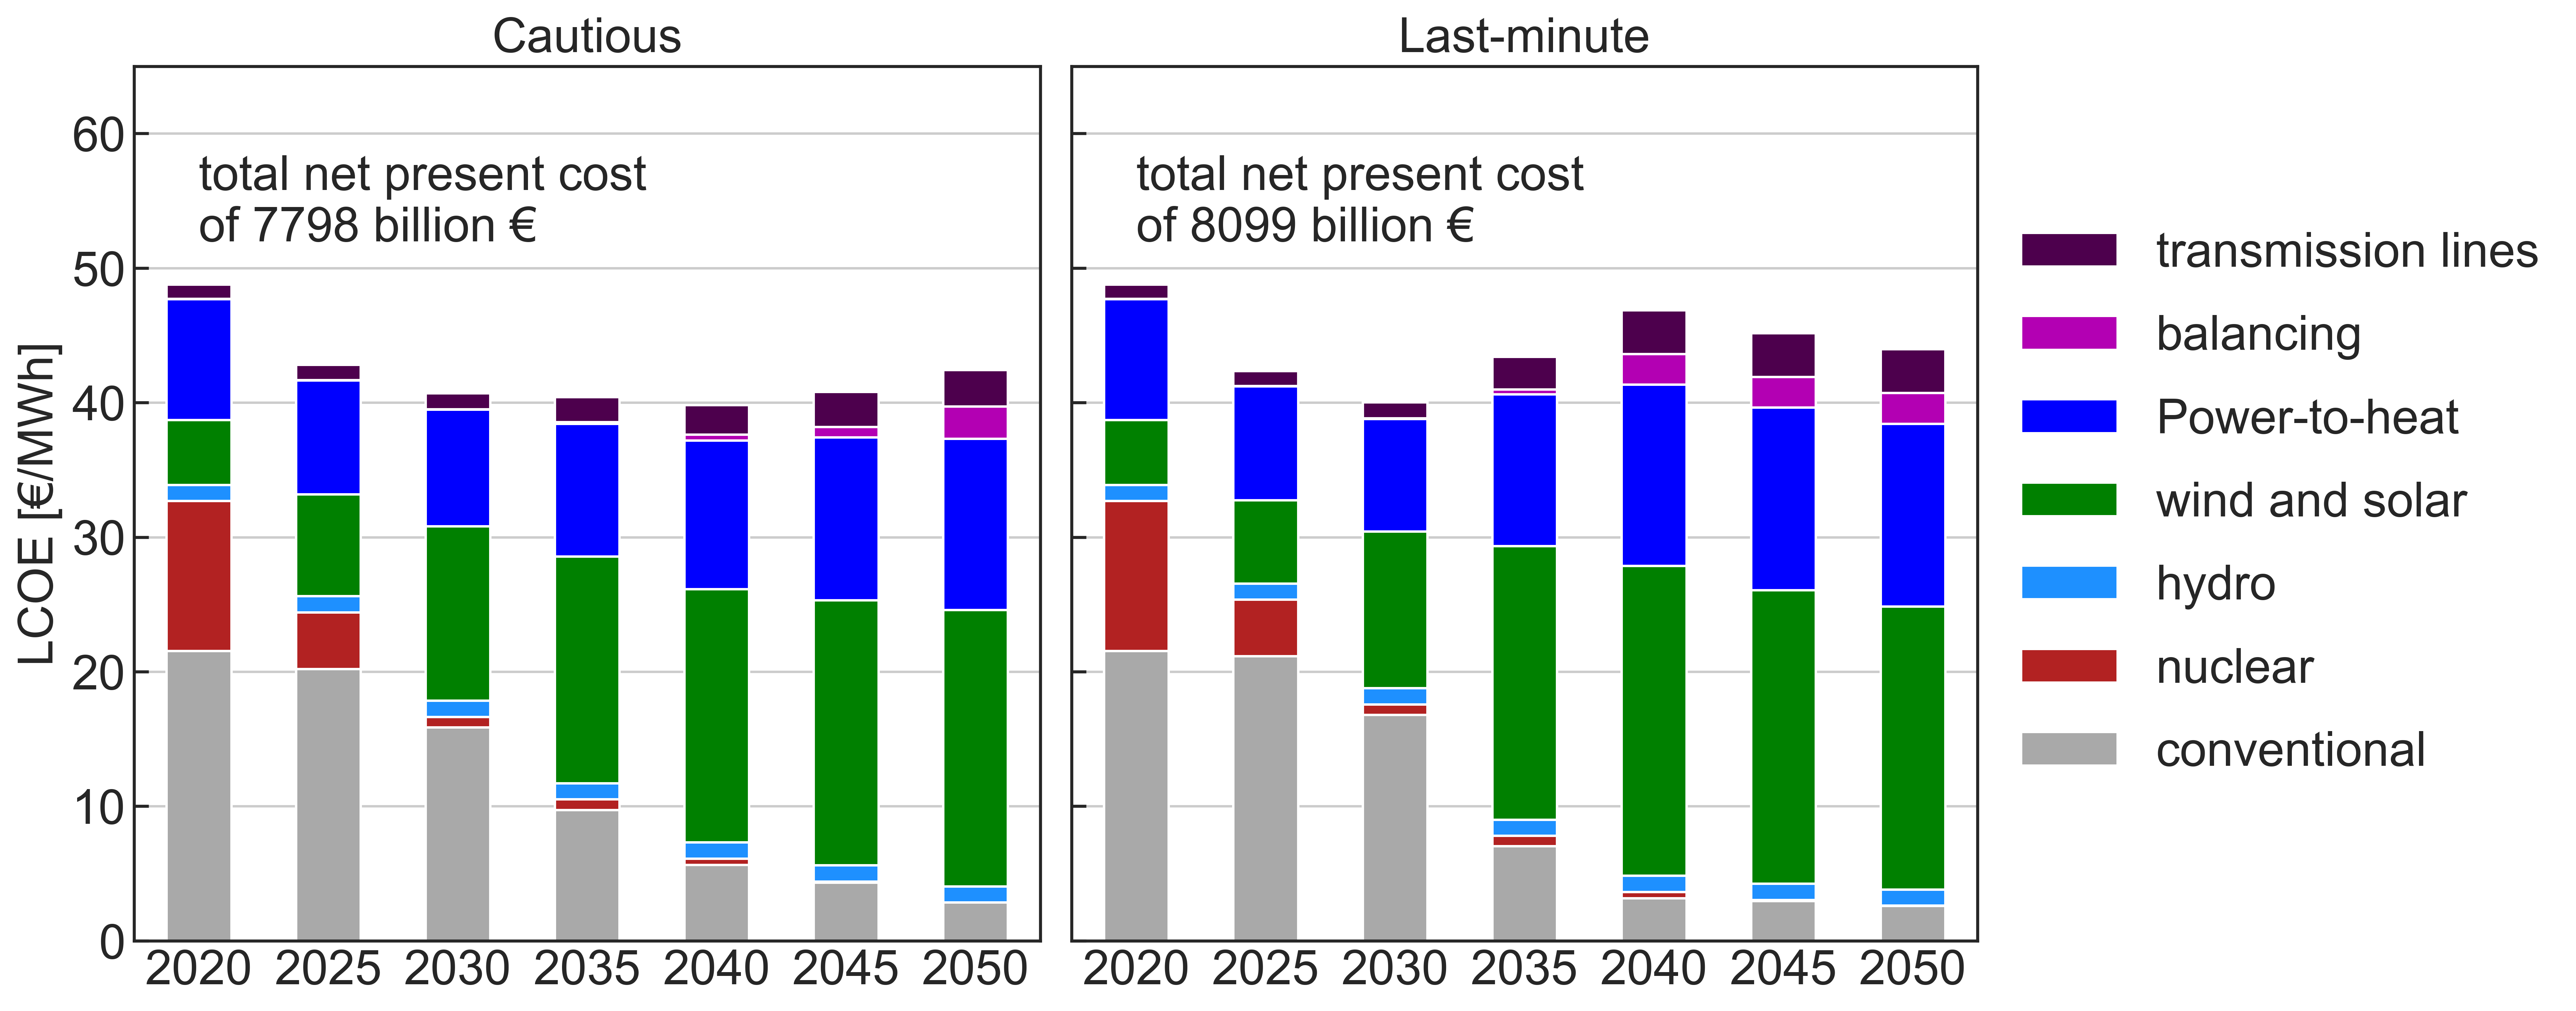
\includegraphics[width=14cm]{figures/LCOE_Base.png}
\caption{Levelized Cost of Energy (LCOE) for the European electricity and heating system throughout transition paths cautious and last-minute shown in Fig. \ref{fig_carbon_budget}. Conventional includes costs associated with coal, lignite, and gas power plants producing electricity as well as gas consumed in gas boilers and CPH units. Power-to-heat category includes costs associated with heat pumps and heat resistors. Balancing includes cost of electric batteries, H$_2$ storage and methanation. } \label{fig_system_cost} 
\end{figure*}

\begin{figure}[!h]
\centering
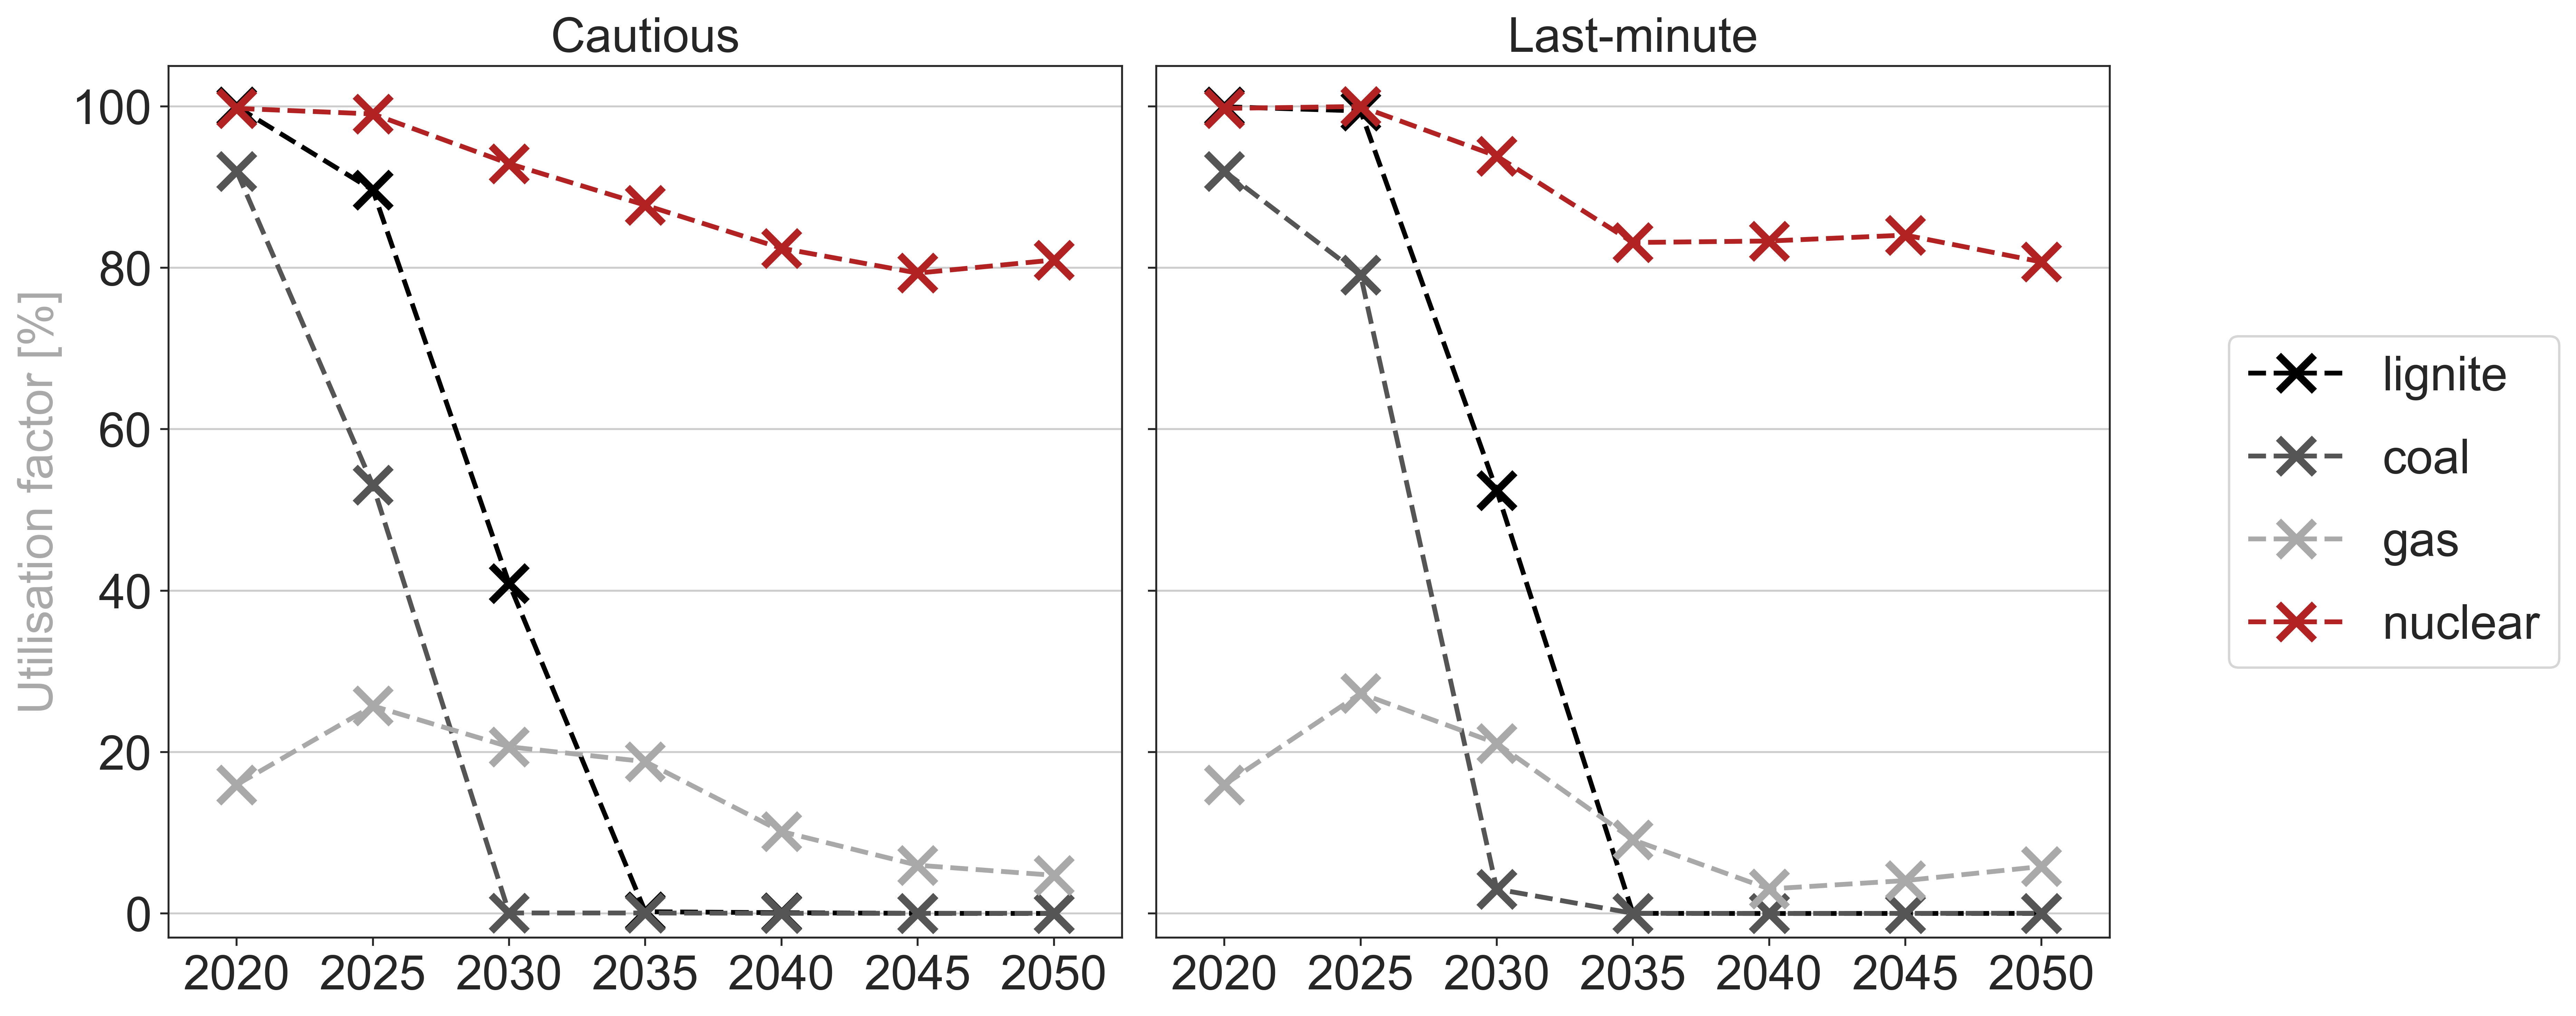
\includegraphics[width=\columnwidth]{figures/utilisation_factors_Base.png}
\caption{Utilisation factors for lignite, coal, gas, and nuclear power plants throughout transition paths shown in Fig. \ref{fig_carbon_budget}. The figure also depicts the percentage of cost that those technologies recover via market revenues. } \label{fig_utilisation_factors} 

\end{figure}

\paragraph{\textbf{Build rates and feasibility of transition paths}} \

During the past decade, several European countries have shown sudden increments in the annual build rate for solar PV, followed by equivalent decrements one or two years later. Italy, Germany, Spain, and UK show clear peaks (see Supplementary Note 4)  due to the combination of a fast cost decrease of the technology and unstable regulatory frameworks whose details are country-specific. These peaks are lethal for local businesses. The sudden shrinkage of annual build capacity results into companies bankruptcy and job loss. The Tortoise transition path requires a smoother evolution of build rates which could better accommodate the cultural, political, and social aspects of the transition \cite{Geels_2017}, see Supplementary Note 5. Although none of the build rates required in the Hare path is technological infeasible, the Tortoise path is more compatible to the inertias in the transition such as required time to modify regulatory frameworks or to educate the necessary labour force. 


\begin{figure*}[!h]
\centering
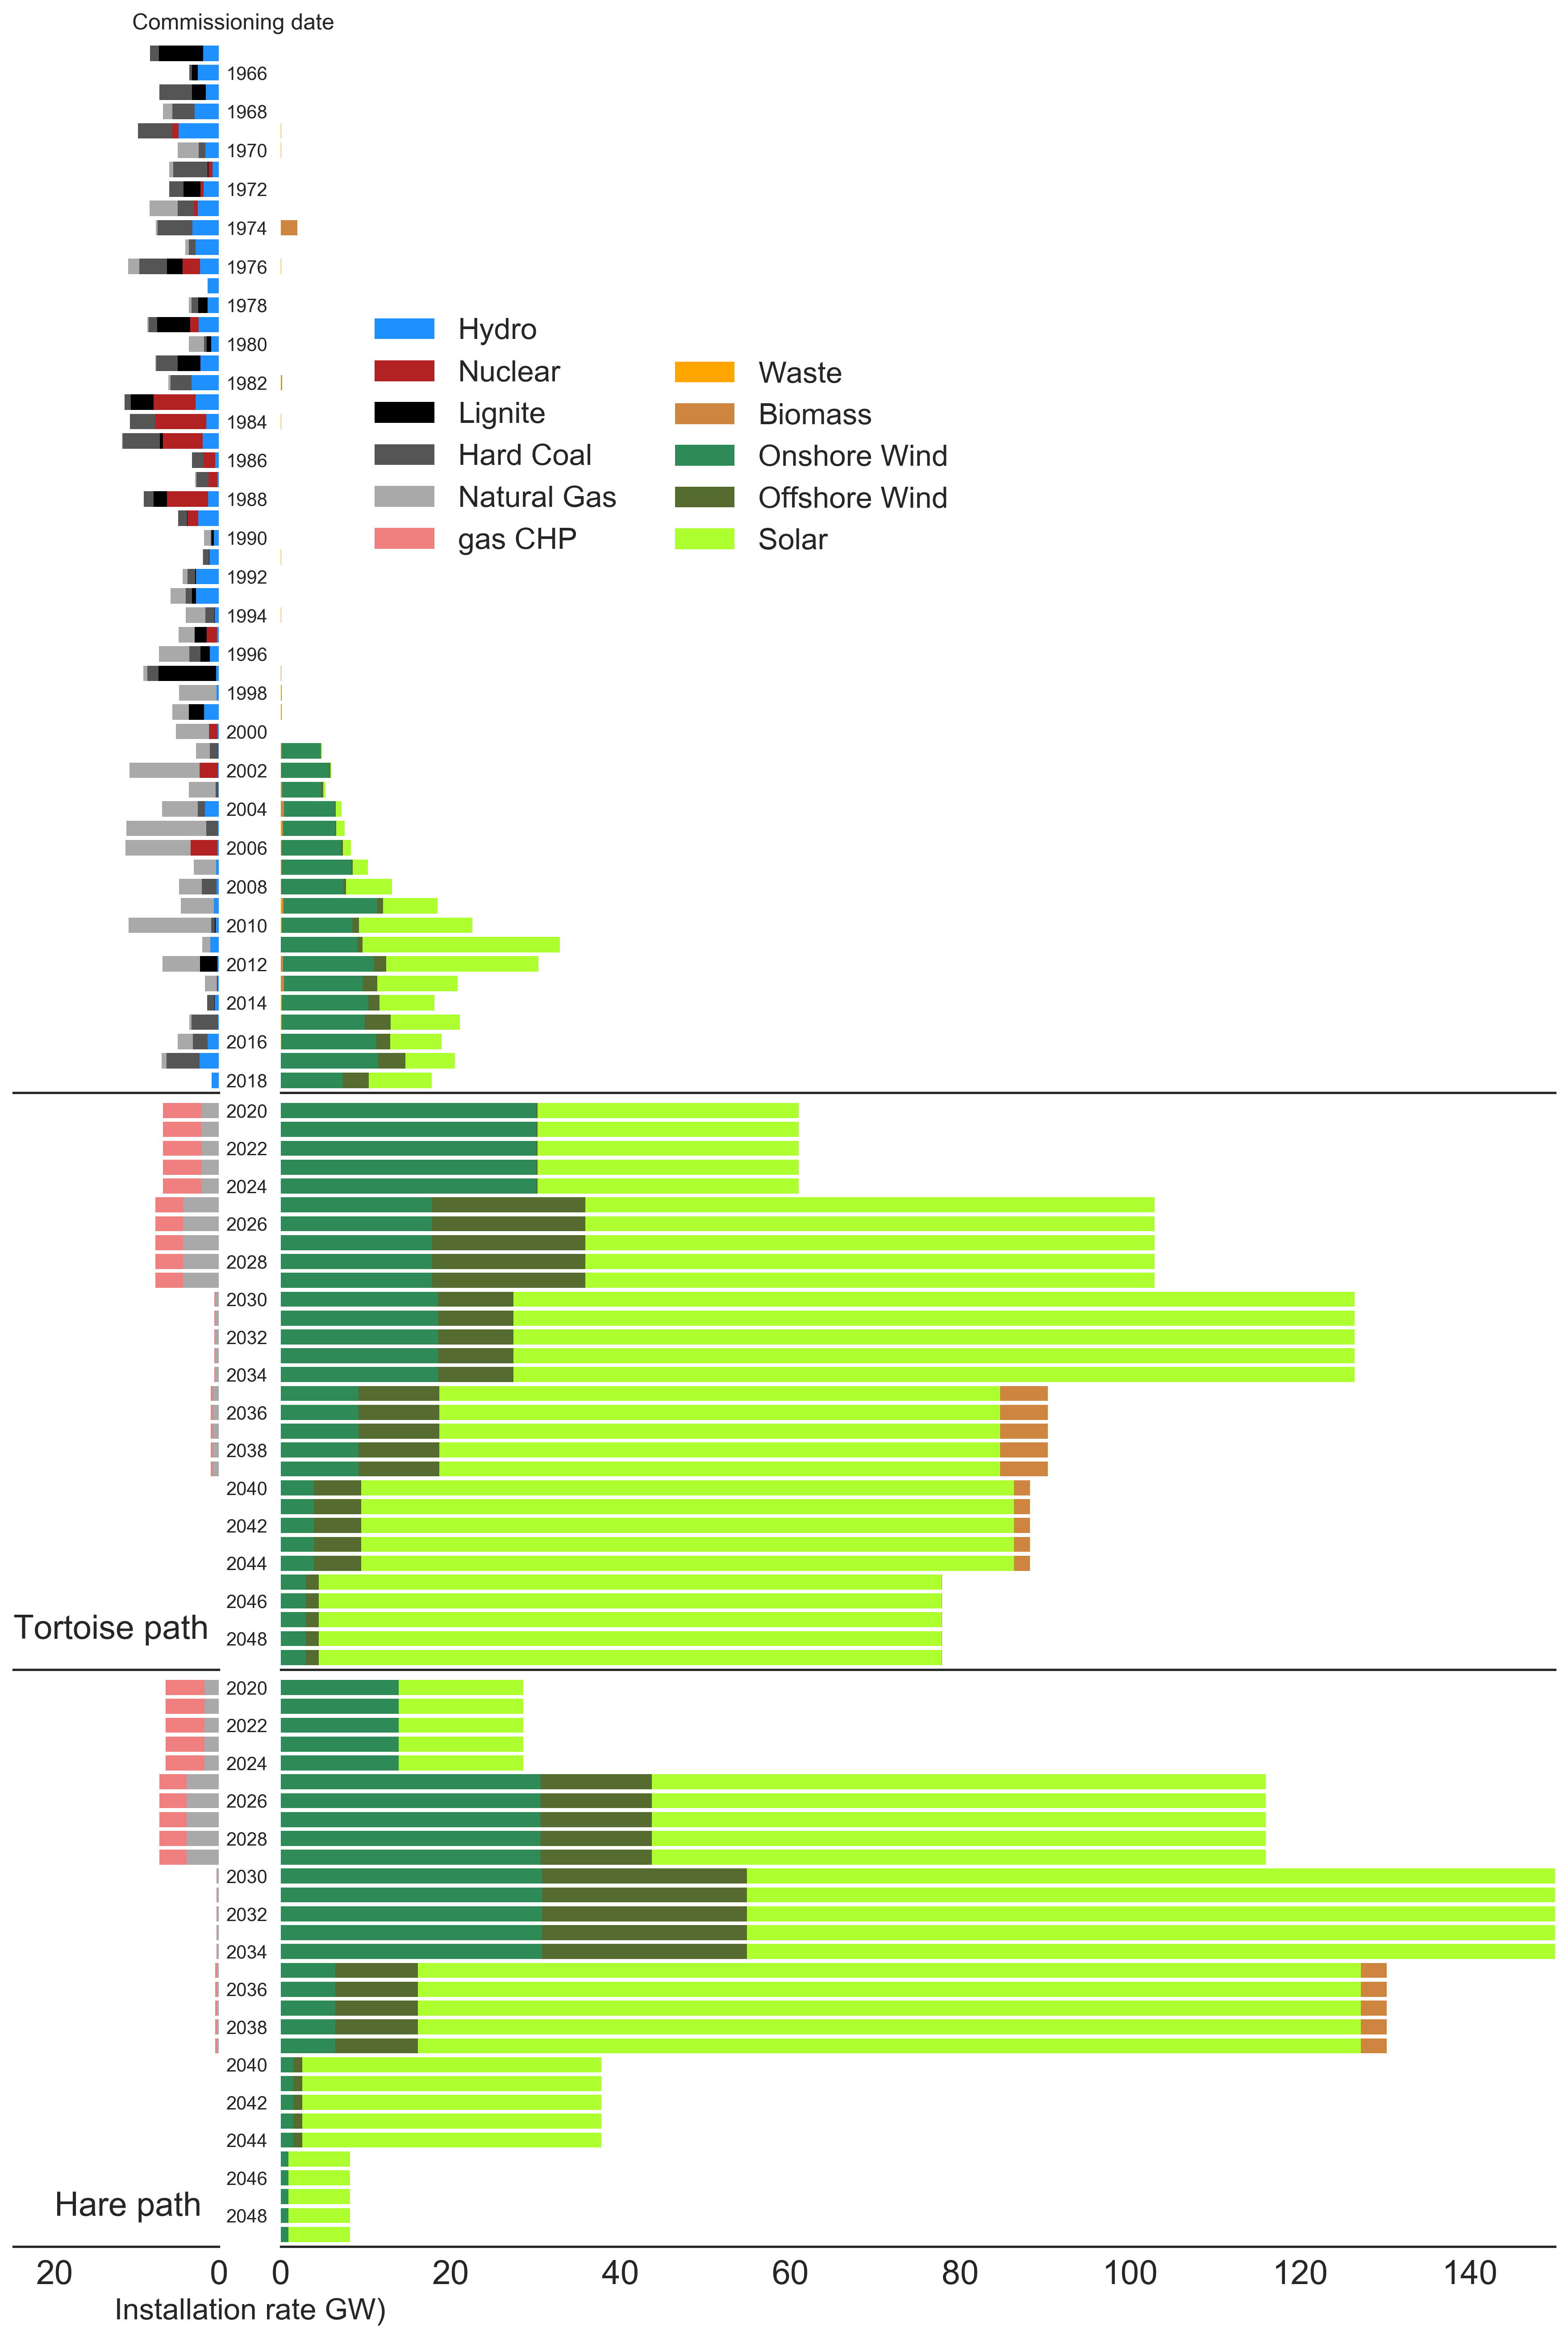
\includegraphics[width=0.8\textwidth]{figures/age_distribution_w_TYNDP.png}
\caption{Age distribution of European power plants in operation \cite{powerplantmatching, IRENA_2019} and required installation in both pathways.} \label{fig_age_distribution} 
\end{figure*}


\begin{figure*}[!h]
\centering
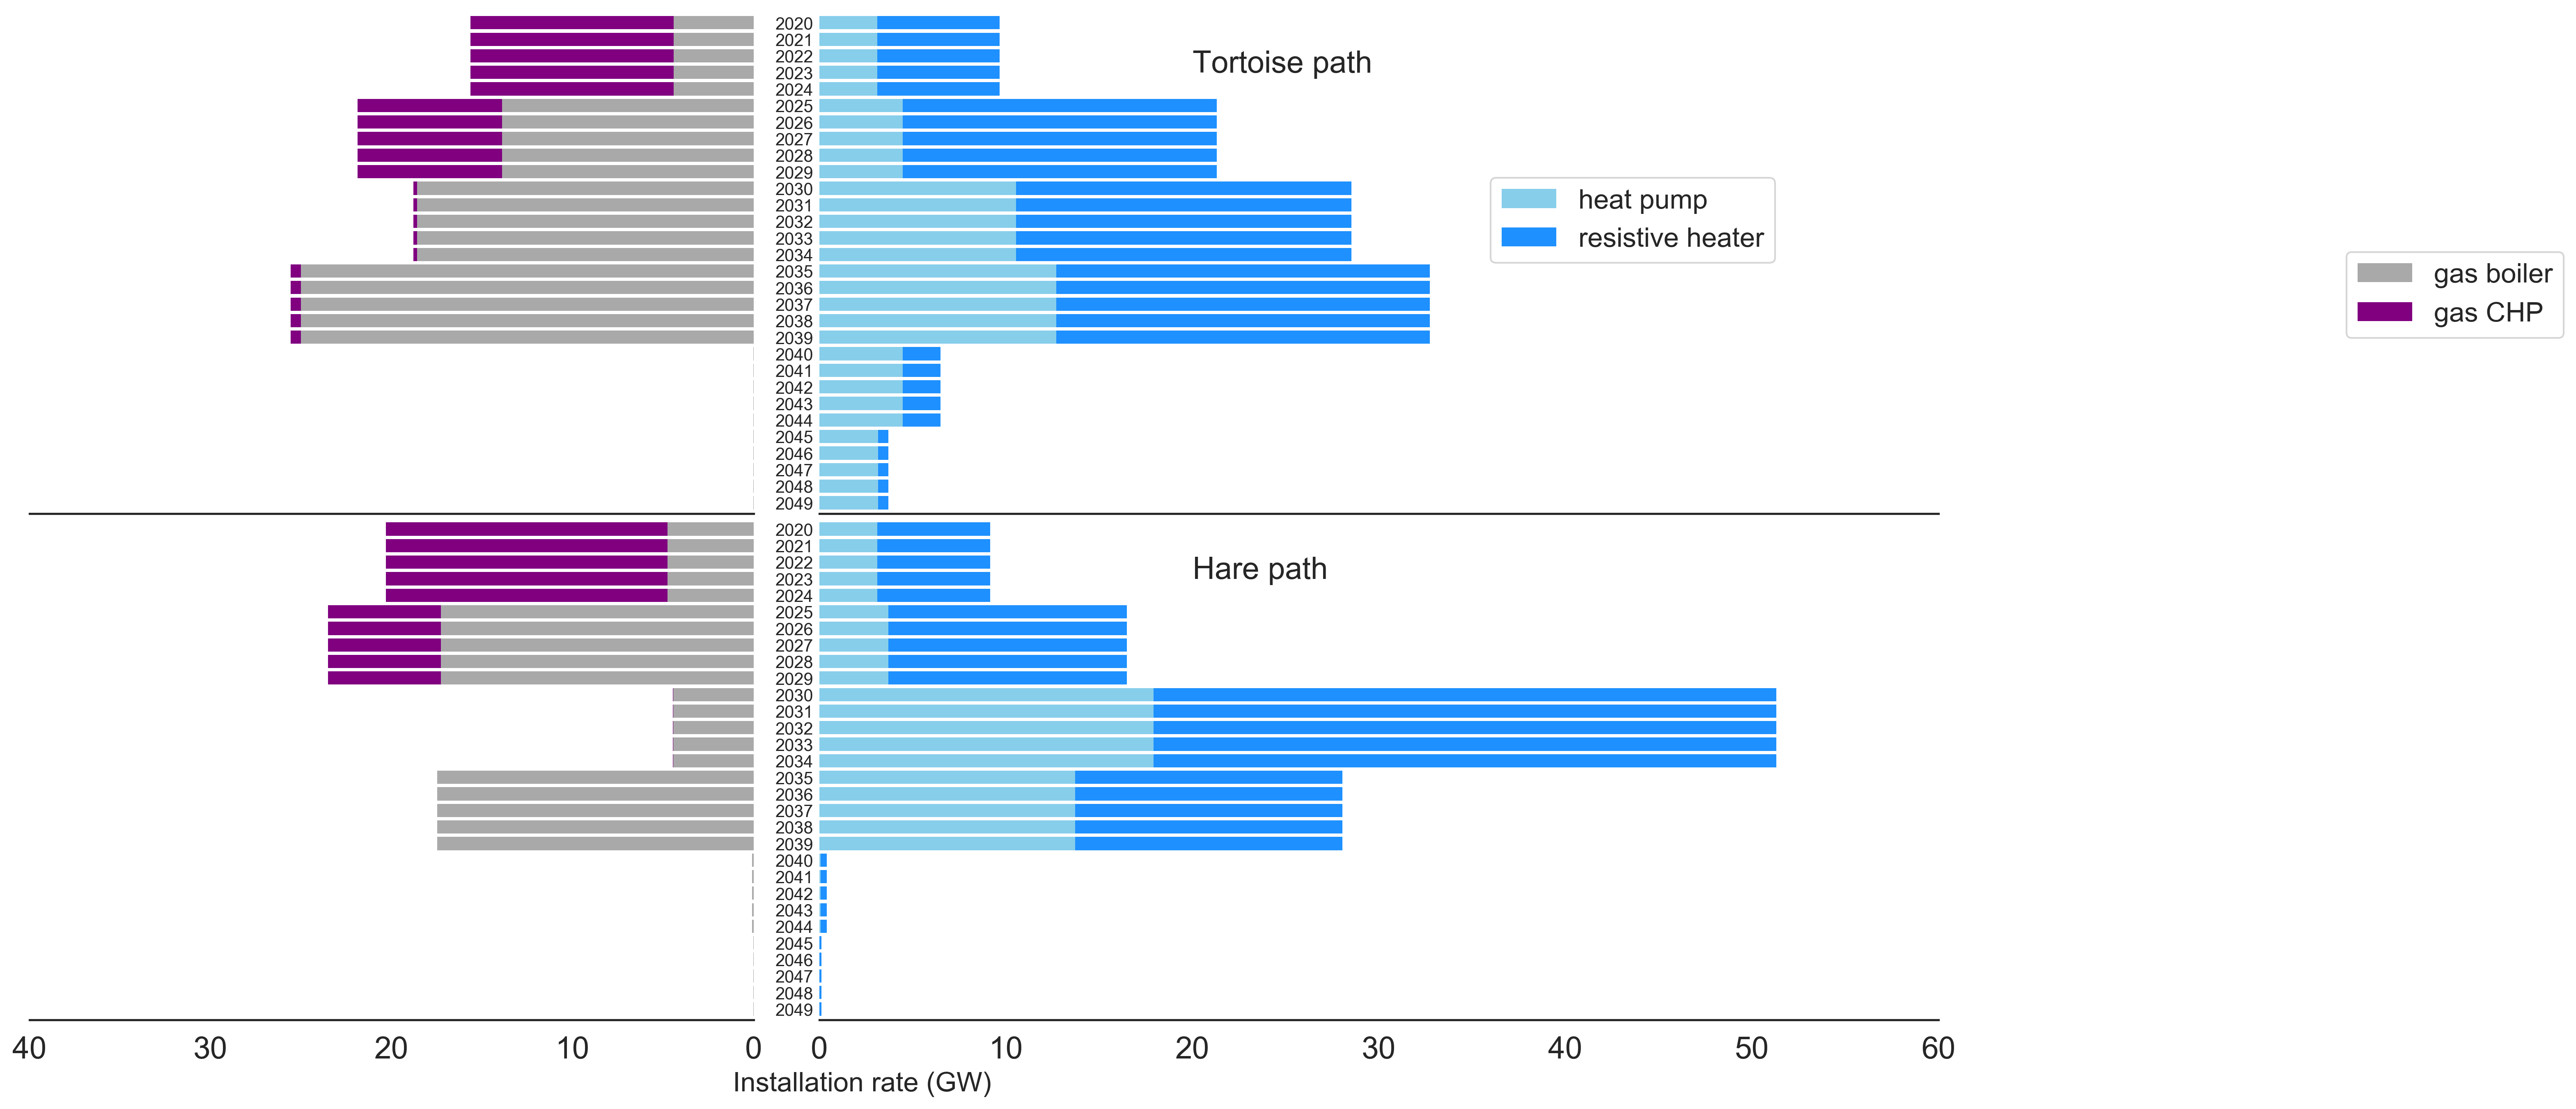
\includegraphics[width=0.8\textwidth]{figures/heating_expansion_w_TYNDP.png}
\caption{Required heating capacities expansion in both pathways.} \label{fig_heating_expansion} 
\end{figure*}

\FloatBarrier

\paragraph{\textbf{Balancing renewable generation}} \

A strong link emerges among renewable generation technologies and balancing strategies. For countries and time steps in which large solar PV capacities are deployed, it is also cost effective to install large battery capacities to smooth the strong daily solar generation pattern. Conversely, onshore and offshore wind capacities require H$_2$ storage and reinforced interconnections to balance wind synoptic fluctuations \cite{Rasmussen_2012, Schlachtberger_2017, Victoria_2019_storage}. This can also be appreciated by looking at the dominant dispatch frequencies unveiled by the Fourier power spectra of the dispatch time series, Fig. \ref{fig_Fourier}. The optimal renewable mix in every country depends on the local resources and the already existing capacities, see Fig. X in Supplementary Note 5. Nevertheless, it should be remarked that the analysis of near-optimal solutions has recently shown that country-specific mixes can vary significantly while keeping the total system cost only slightly higher than the minimum \cite{Neumann_2019}. 

\begin{figure}[!h]
\centering
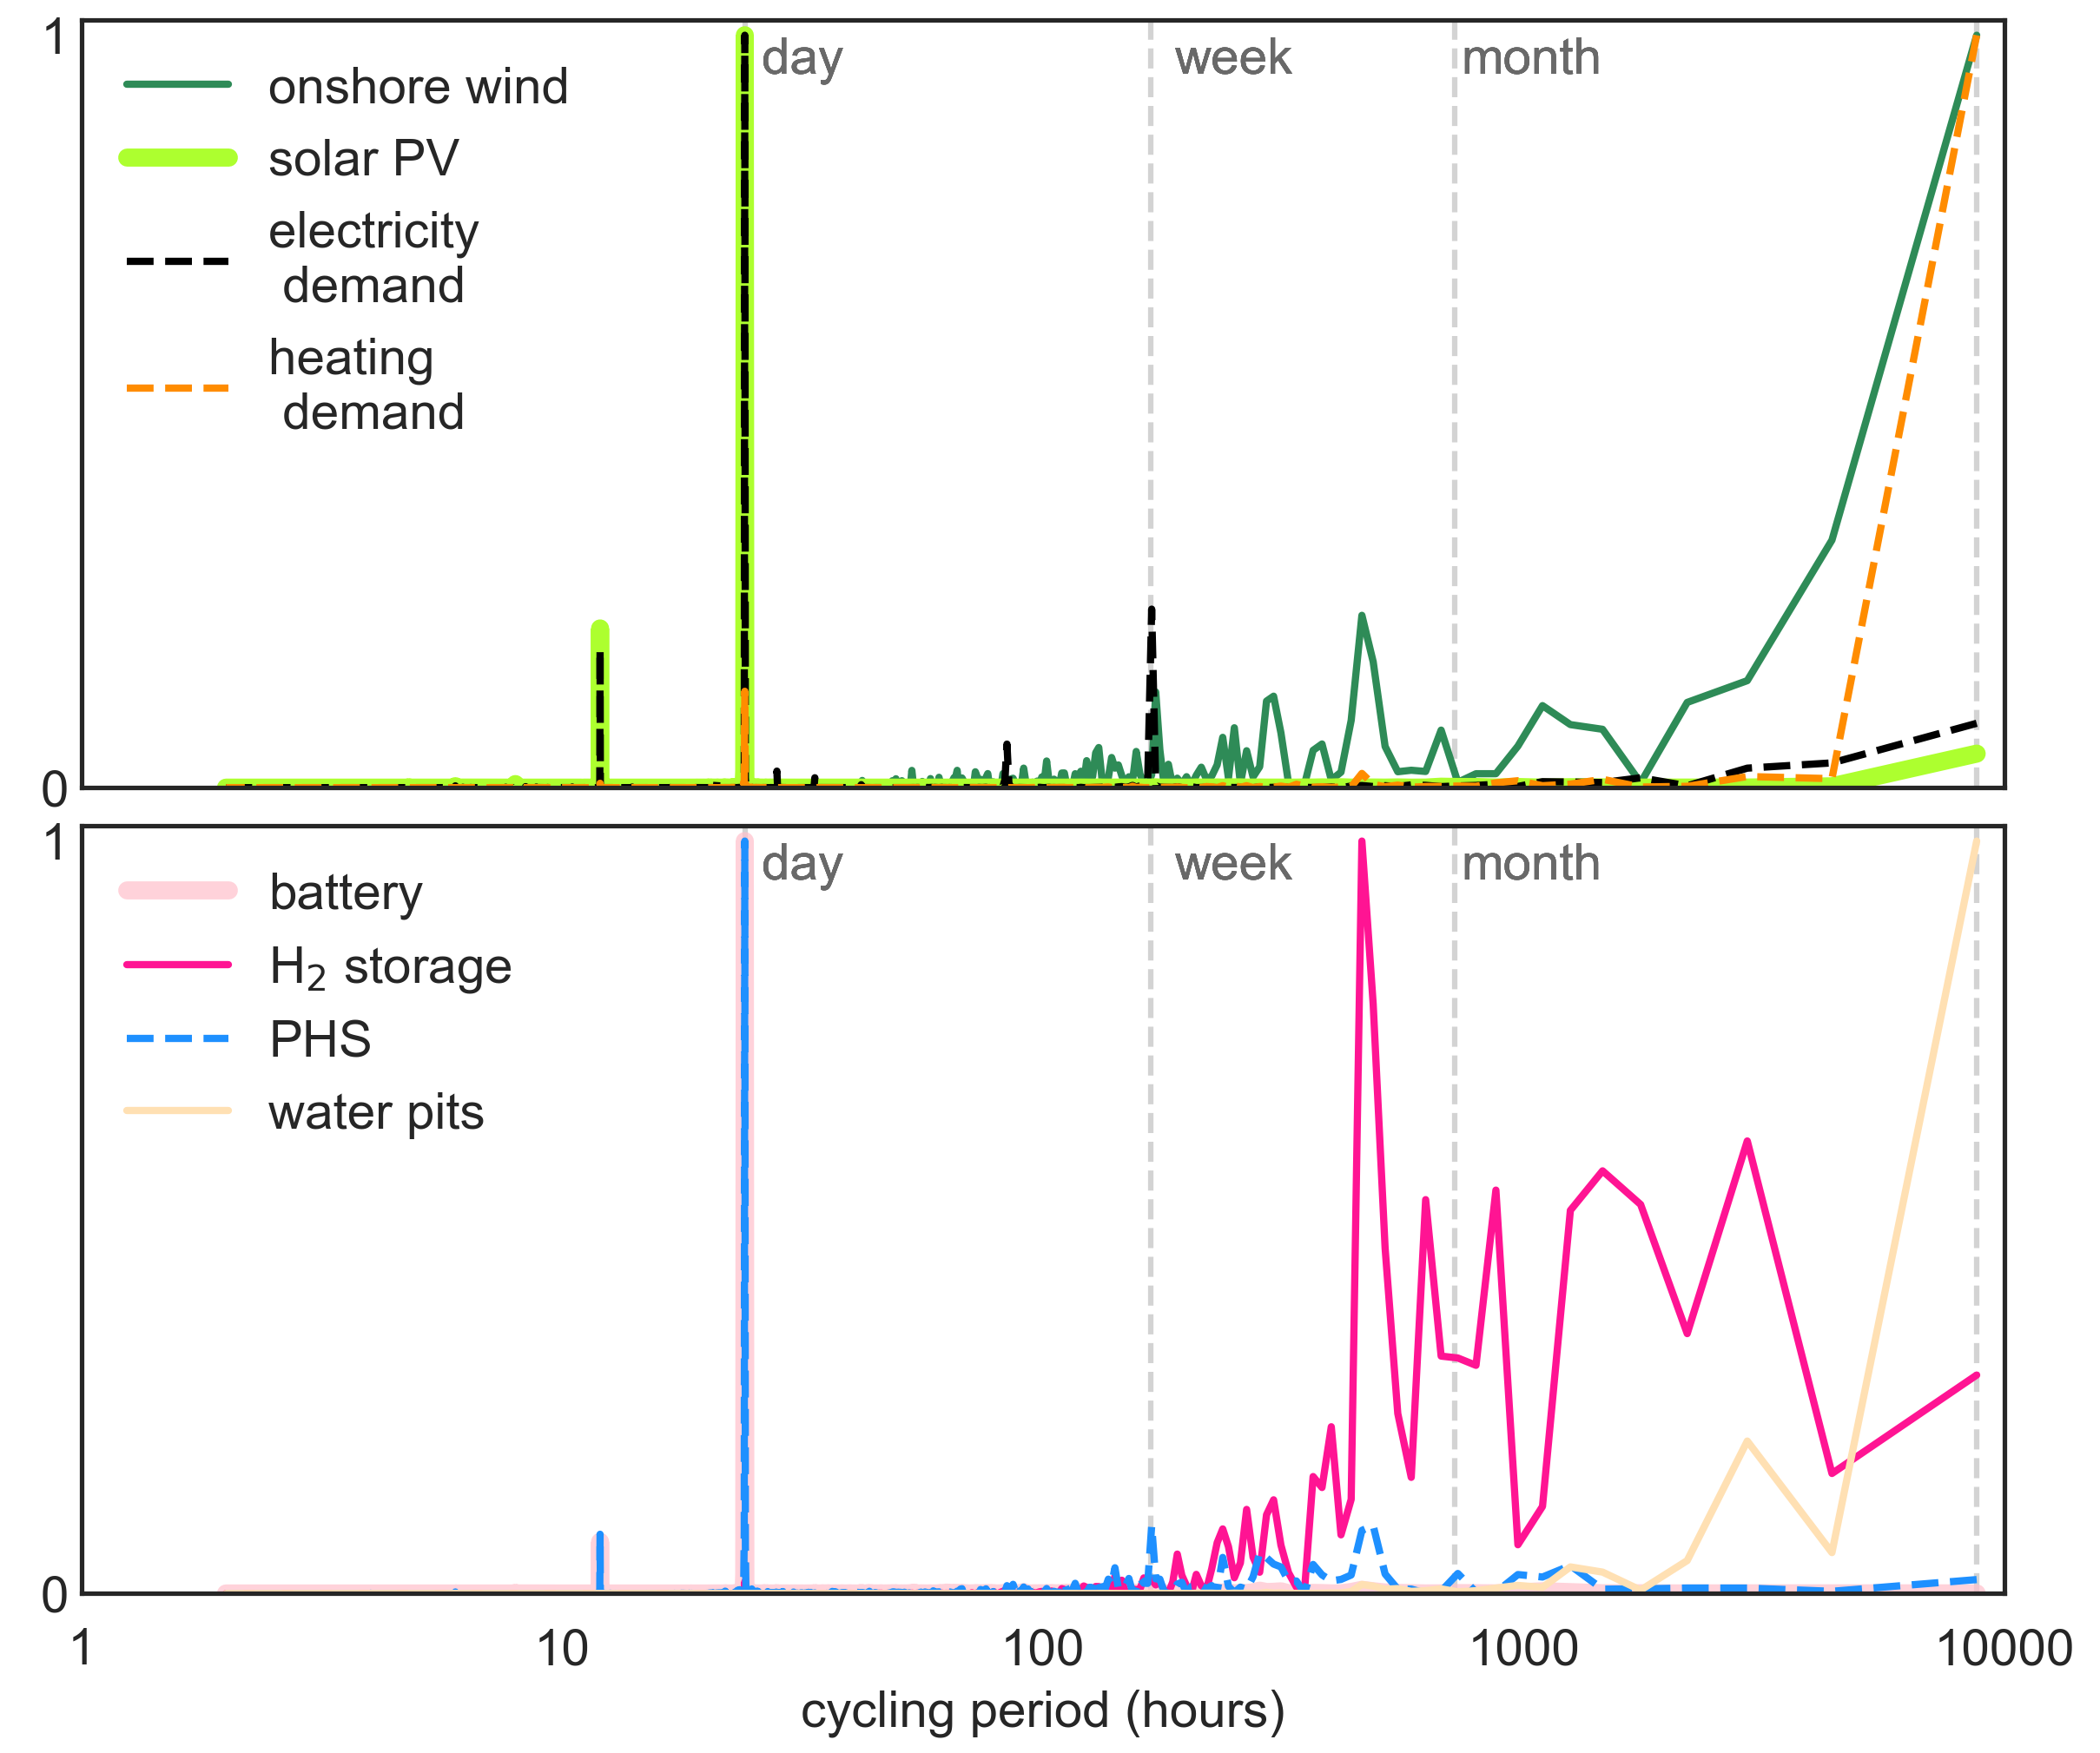
\includegraphics[width=\columnwidth]{figures/Fourier.png}
\caption{Fourier power spectra of wind and solar PV generation, electricity and heating demand, as well as storage technologies dispatch time series.} \label{fig_Fourier} 
\end{figure}

\FloatBarrier
 
\paragraph{\textbf{Policy incentives are needed}} \

CO$_2$ prices much higher than those historically attained in the ETS market are required throughout the transition, Fig. \ref{fig_co2price}. Several remarks are worth it. First, CO$_2$ price is impacted by the model assumptions and lower values could be obtained if, for example, a lower cost was assumed for biomass. Second, due to its large seasonal variation, decarbonisation of the heating sector is known to require higher CO$_2$ prices than the power system, mainly to push into the system high-efficiency but capital-expensive technologies such as heat pumps \cite{Brown_2018, Victoria_2019_storage}. Third, CO$_2$ prices are only and indication of the price gap between polluting and clean technologies, and several policies can be established to fill that gap. Among others, sector-specific CO$_2$ taxes, auctions for renewable capacity that reduce the risk, and consequently the WACC and LCOE of the technology, or regulatory frameworks that incentivise the required technologies such those promoting household PV systems or ensure the competitiveness of district heating systems.

\begin{figure}[!h]
\centering
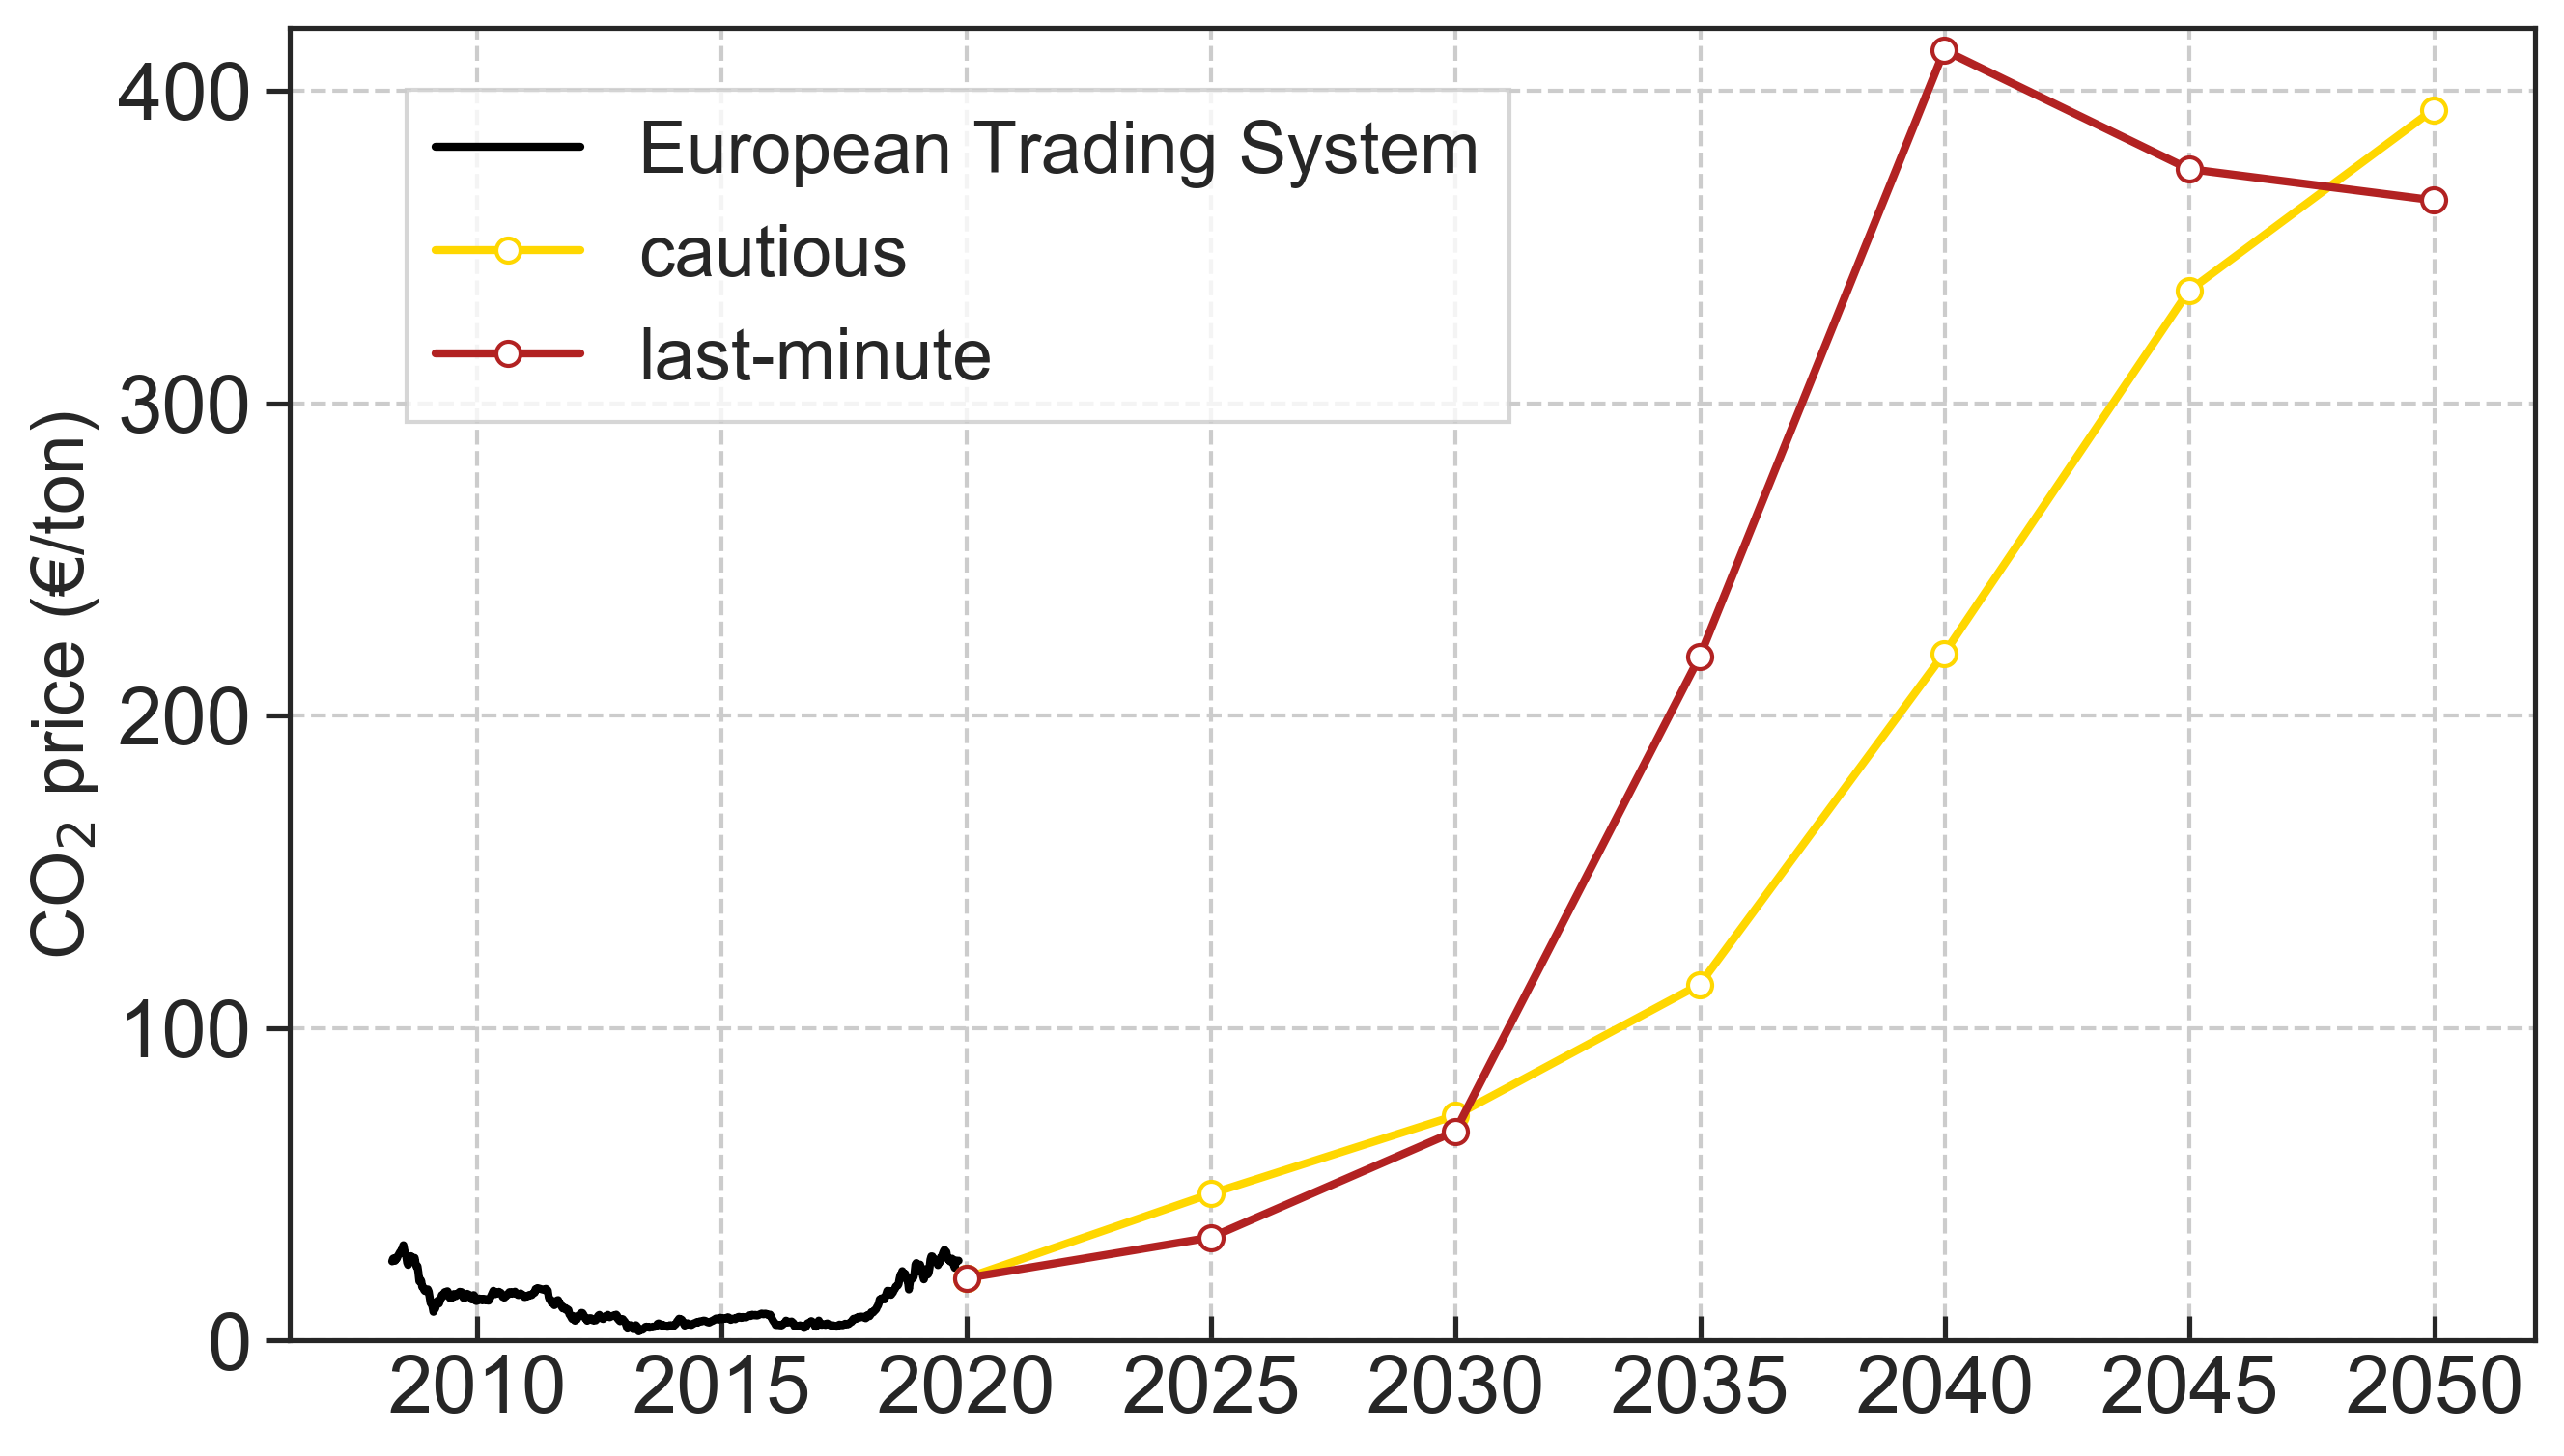
\includegraphics[width=\columnwidth]{figures/co2_price.png}
\caption{Historical evolution of CO$_2$ price in the European Trading System \cite{ETS} and required CO$_2$ price obtained from the model throughout transition paths shown in Fig. \ref{fig_carbon_budget}} \label{fig_co2price} 
\end{figure}


\paragraph{\textbf{The challenging decarbonisation of the heating sector}} \

District heating has proven to be extremely useful to decarbonise the heating sector. It allows cheaper centralised technologies such as heat pumps and CHP units, and makes possible a fast conversion because it is easier to substitute one central heating unit that a myriad of individual domestic systems. On the top of that, district heating enables long-term thermal energy storage, via cheap large water pits, Fig.\ref{fig_Fourier}, that help balancing the large seasonal variation of heating demand, Supplementary Note 7. In the initial paths, district heating penetration in every country was kept fixed at its value in 2015 \cite{DH_penetration} throughout the entire path. When they are assumed to expand linearly so that all the urban heat demand in every country is supplied via district heating, cumulative system cost for the Tortoise path reduces by 250 B\EUR. The additional cost of extending and maintaining the required district heating network can be estimated in 10 B\EUR/year \cite{Brown_2018} which roughly offsets the gains. However, including in the calculation the avoided expansion of gas distribution networks when district heating is deployed, makes this option clearly cheaper. 

\paragraph{\textbf{Impact of building retrofitting}} \


\textcolor[rgb]{1,0,0}{TODO: Run cautious path including path for reduction of heating demand, e.g. 2\% per year and write paragraph discussing the results}


\paragraph{\textbf{Transitioning without grid expansion}} \

When the model is allowed to optimized transmission capacities after 2030 together with the generation and storage assets, the optimal configuration in 2050 includes transmission volume approximately three times larger than that of 2030.  Although, the cumulative system cost is 84 B€ lower it is unclear that it compensates the social acceptance issues associated with increasing transmission. A reinforced network favours the penetration of onshore and offshore wind whose capacities can increase in regions where the resource is high. The wind generation can be easily transported and smoothed by the grid. Lower hydrogen storage capacities are also needed due to the network contribution to wind balancing. 




\paragraph{\textbf{Coupling the transport sector}} \

\textcolor[rgb]{1,0,0}{TODO: Run cautious path including path representing the electrification of the transport sector and write paragraph discussing the results.}

%\paragraph{\textbf{Early action allows room for decision-making later}} \
%\textcolor[rgb]{1,0,0}{TODO: Run cautious path banning the use of coal and lignite after 2025/2030 and write paragraph discussing the results}

%\paragraph{\textbf{Heterogeneity among European countries}} \
%\textcolor[rgb]{1,0,0}{TODO: Discuss final system configuration obtained as a result of the path vs. greenfield optimization in 2050.}

%\begin{footnotesize}
\section{Methods}

The system configuration is optimised by minimising annualised system cost in every time step (one every 5 years), under the global CO$_2$ emissions cap imposed by the transition path under analysis (Fig. \ref{fig_carbon_budget}). This can be considered a myopic approach since the optimisation has no information about the future. The cumulative CO$_2$ emissions for all the different transition paths is equal to a carbon budget of 21 GtCO$_2$. In every time step, generation, storage, and transmission capacities in every country are optimised assuming perfect competition and foresight as well as long-term market equilibrium. Besides the global CO$_2$ emission cap, other constraints such as the demand-supply balance in every node, and the maximum power flowing through the links are imposed to ensure the feasibility of the solution, see Supplementary Note 6. \

We use a one-node-per-country network, including 30 countries corresponding to the 28 European Union member states as of 2018 excluding Malta and Cyprus but including Norway, Switzerland, Bosnia-Herzegovina, and Serbia (Fig. \textcolor[rgb]{1,0,0}{X} in the Supplementary Notes). Countries are connected by High Voltage Direct Current (HVDC) links whose capacities can be expanded if it is cost-effective. In the power sector, electricity can be supplied by onshore and offshore wind, solar photovoltaics (PV), hydroelectricity, Open Cycle Gas Turbines (OCGT), Combined Cycle Gas Turbines (CCGT), Coal, Lignite, and Nuclear power plants, and Combined Heat and Power (CHP) units using gas, coal or biomass. Electricity can be stored using Pumped Hydro Storage (PHS), static electric batteries, and hydrogen storage. Hydrogen is produced via electrolysers and converted back into electricity using fuel cells. Methane can be produced by combining Direct Air Captured (DAC) CO$_2$ and electrolysed-H$_2$ in the Sabatier reaction.  
%Historical time series from 2015 are used to represent electricity demand. Future demands increments in our model are captured via heat demands or transport demand when included.  
Heating demand is split into urban heating, corresponding to regions whose population density allows centralised solution, and rural heating where only individual solutions are allowed. Heating can be supplied via central heat pumps, heat resistors, gas boilers, solar collectors, and CHP units for urban regions, while only individual heat pumps, electric boilers, and gas boilers can be used in rural areas. Centralised and individual thermal energy storage can also be installed. A detailed description of all the sector is provided in the Supplementary Note 7. \

Costs assumed for the different technologies depend on time (Supplementary Note 8) but not on the cumulative installed capacity since we assume that they will be influenced by the forecast global installation rates and learning curves. The financial discount rate applied to annualise costs is equal to 7\% for every technology and country. Although it can be strongly impacted by the maturity of a technology, including the country-specific experience of it, and the rating of a country \cite{Egli_2019}, we assumed European countries to be similar enough to use a constant discount rate. For decentral solutions, such rooftop PV, heat resistors and gas boilers, discount rate equal to 4\% is assumed. The already installed capacities, \textit{i.e.} existing capacities in 2020 or capacities installed in a previous year whose life time has not concluded, are exogenously included in the model. For every time step, the total system cost includes two components. First, the costs of newly installed assets, which exactly recover their investment by market revenues. Second, the stranded costs for the exogenously fixed capacities. They are determined as the difference between the annualised costs and the revenues that those assets get from the market.  To estimate the cumulative cost of every transition path, the annualised cost for all year are added assuming a social discount rate of 2\%. This rate represents the value at which we, as European society, discount investments in far-future years when comparing them with present investments. We have selected a social discount rate of 2\%, which is similar to the inflation rate in the European Union, that averaged 2.4\% in the past 20 years. It is worth remarking that the cumulative cost remains lower for the last-minute path provided that discount rates lower than 11\% are assumed. The CO$_2$ price is not an input to the model, but a result that is obtained via the Lagrange/Karush-Kuhn-Tucker multiplier associated with the global CO$_2$ constrain. 
%\end{footnotesize}

\section{Data availability and code availability}

\section{References}
\bibliography{bib_transition}

\end{document}